% The "%" character denotes a comment
% This file was written by Nathan Moore, Winona State University
% as a template for how lab reports might be written in LaTeX.
% style choices originally come from the American Journal of Physics's
% sample submission file, http://ajp.dickinson.edu/Contributors/manFormat.html
%
%
\documentclass[prb,preprint]{revtex4-1}
\usepackage{amsmath}  % needed for \tfrac, \bmatrix, etc.
\usepackage{amsfonts} % needed for bold Greek, Fraktur, and blackboard bold
\usepackage{graphicx} % needed for figures

%these are some macros (shortcuts)
\newcommand{\bea}{\begin{eqnarray}}
\newcommand{\eea}{\end{eqnarray}}
\newcommand{\be}{\begin{equation}}
\newcommand{\ee}{\end{equation}}

\begin{document}

\title{Digital Circuits Lab 08: 4-bit Full Adder}
\author{Adam Stammer}
%\email{adam.stammer@go.winona.edu}

\date{\today}

%if you include an abstract, it goes here
\begin{abstract}
To test our binary calculation skills, and build our understanding of verilog, we implemented a 4 bit full adder circuit using the switches as input and LEDs as output. From there we sought to output our sum value to the 7 segment display in decimal. Due to the complexities of converting from binary to decimal representation, we elected to only display a single digit on the 7-segment display, limiting our meaningful sum output to that of single digit numbers.
\end{abstract}

\maketitle


%These are my general reccomendations for an undergraduate lab report in Physics. 
%
%\textbf{Purpose}
%The lab report should start with a purpose statement.  Briefly 
%provide the necessary background and explain what problem your are trying to 
%solve/investigate.
%
%\textbf{Conclusions} Don't be coy, cut to the point right away and state what you found. This should be breif.
%
%\textbf{Theory} We never just measure stuff in Physics.  There's always a 
%theoretical idea behind the measurement we're making.  Explain  the ideas 
%behind your work, starting at the level of a successful Physics 221/222 
%student.
%
%\textbf{Data} Sketch out, in words and pictures, the apparatus you used to take data.  Report the data, graphically, if possible, and state the uncertainties  in your measurement.  Don't provide pages of computer printout here. Data tables shouldn't be your first choice when it comes to communicating your measurements.\cite{Tufte}
%
%\textbf{Analysis} With data presented, describe how the theory agrees/disagrees with 
%the data you took.  Normally this is accomplished with a fit line (or math 
%model) that is interpreted.
%
%\textbf{Limitations and Recommendations} Every measurement has limitations and it is only honest to report them to the reader.  ``Human Error'' is a meaningless statement.  After your analysis is complete, revisit the purpose statement.  This is the place to more forcefully argue your conclusions.    
%
%Notes: 
%Writing in the first person, eg ``I" or ``We," is fine.
%
%\newpage
%\textbf{Example Lab Report:}

\section{Theory}
We know that a full adder circuit takes in two bits to be added together with an additional carry-in bit. The output falls into two bits, one for the carry-out bit, and the other for the sum bit. Considering the small number of possible inputs, it's easy to write out each possibility and build a full truth table from that. The resulting truth table can be seen below.

\begin{displaymath}
\begin{array}{|c c c|c c|}
% |c c|c| means that there are three columns in the table and
% a vertical bar ’|’ will be printed on the left and right borders,
% and between the second and the third columns.
% The letter ’c’ means the value will be centered within the column,
% letter ’l’, left-aligned, and ’r’, right-aligned.
c_{in} & q & p & c_{out} & sum\\ 
% Use & to separate the columns
\hline  
% Put a horizontal line between the table header and the rest.
0 & 0 & 0 & 0 & 0\\
0 & 0 & 1 & 0 & 1\\
0 & 1 & 0 & 0 & 1\\
0 & 1 & 1 & 1 & 0\\
1 & 0 & 0 & 0 & 1\\
1 & 0 & 1 & 1 & 0\\
1 & 1 & 0 & 1 & 0\\
1 & 1 & 1 & 1 & 1\\
\end{array}
\end{displaymath}

This truth table can be made into a rather simple karnough map to extract the logic to achieve this calculation. It ultimately ends in the following.

\begin{equation}
c_{out} =  A \land (B \lor C) \lor (B \land C)
\end{equation}

\begin{equation}
sum = (\lnot A \land \lnot B \land C) \lor (\lnot A \land B \land \lnot C) \lor (A \land B \land C) \lor (A \land \lnot B \land \lnot C)
\end{equation}

With this it wasn't too hard to build a module with the inputs and outputs mentioned above that just did these two logical calculations. By using an array of wires to store the carry bits, the modules can then be strung together one bit at a time. In this instance we made a 4 bit full adder, so the output could be up to 5 bits in size, as $15 + 15 = 30$ and 30 requires 5 bits to store. The fifth bit is just the $c_{out}$ of the last adder.

If we then store the sum values in a wire array too, we can connect this output to 5 of the onboard LEDs, and pipe this sum value as one unit to another module made to display the number on the 7 segment display.

Converting from binary to decimal is nothing new, but generally requires the use of division and modulus, two features that we could build as separate arithmetic logic units, but not something I thought worth investing in for this lab. I did however try to do so in the next lab (8).

An alternative to this is to treat the multiple digits as one giant output register. A multi-digit truth table based on the sum value could be computed and logic statements pulled from it, but this seemed an even more daunting task and quite frankly less practical than the solution above.

So I instead just displayed the first digit of output to the screen, without any error corrections passed the digit 9. The boards manual provided the relevant truth table for the pins, and a simple case statement made conversion of a 4 bit binary number to the 8 bit code displaying the decimal number on the 7-segment displays not too bad. This also avoided the refreshing logic needed to display more than one digit on the display at a time.

%\begin{figure}[ht]
%\centering
%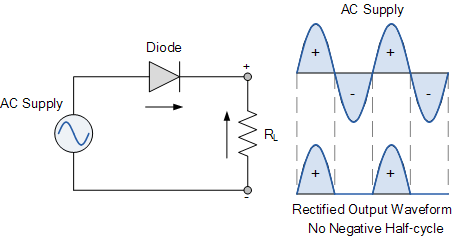
\includegraphics[width=4in]{hwr.png}
%\caption{Half Wave Rectifier Circuit (Credit: www.electronics-tutorials.ws)}
%\label{fig1}
%\end{figure}


%\begin{thebibliography}{99}
% The numeral (here 99) in curly braces is nominally the number of entries in
% the bibliography. It's supposed to affect the amount of space around the
% numerical labels, so only the number of digits should matter--and even that
% seems to make no discernible difference.
%Not Requested
%\end{thebibliography}

\end{document}
